% file: reasoning_case.tex

\begin{ReasoningBox}[title=Perception Error] % 可以通过 title 参数修改标题
    % --- 第一部分：问题描述与图片 ---
    % \begin{minipage}[t]{0.58\textwidth}
    \begin{wrapfigure}{r}{0.5\textwidth}
        \centering
        % wrapfigure 通常顶部会有多余空白，使用负 vspace 向上提，让图片和第一行文字对齐
        \vspace{-15pt} 
        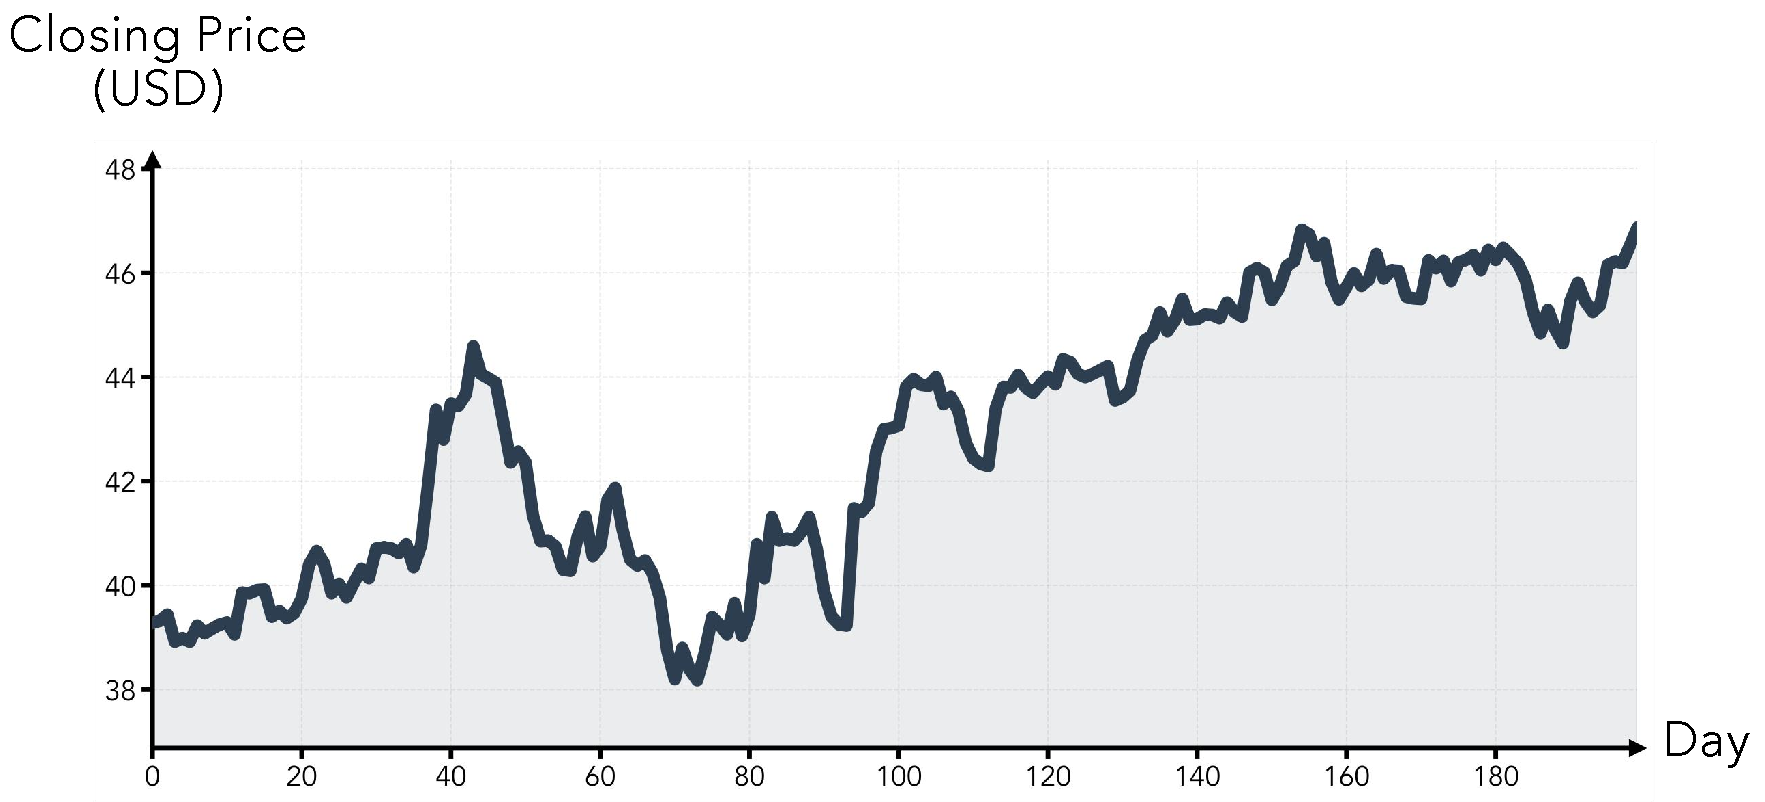
\includegraphics[width=\linewidth]{blocks/case_study_figs/perception_error.pdf}
        % 调整底部的留白
        \vspace{-20pt}
    \end{wrapfigure}
        \textbf{Question:} You are a quantitative analyst backtesting several trading strategies. Here are the five strategies you're evaluating:
        
        (A) SMA Crossover (20/50): Buys when the 20-day moving average crosses above the 50-day moving average, sells when it crosses below.
        (B) MACD (12/26/9): Buys when the MACD line crosses above the signal line, sells when it crosses below.
        (C) RSI (14, 30/70): Buys when RSI falls below 30 (oversold condition), sells when RSI rises above 70 (overbought condition).
        (D) Bollinger Bands (20, $2\sigma$): Buys when price falls below the lower band ($P < \mu - 2\sigma$), sells when price rises above the upper band ($P > \mu + 2\sigma$).
        (E) Buy and Hold: Enters the position at the beginning and holds it for the entire period.
        You have backtested these strategies on the provided price series with an initial capital of \$10,000 and a transaction cost of 0.1\% per trade. Based on the price data provided and standard technical analysis principles, which strategy would you expect to achieve the best Maximum Drawdown (MDD)?
    % \end{minipage}%
    % \hfill
    

    \vspace{0.5em}

    % --- 第二部分：选项 ---
    \textbf{Answer Choices:} (A) SMA Crossover, (B) MACD, (C) RSI, (D) Bollinger Bands, (E) Buy and Hold \\
    \textbf{Correct Answer:} \textcolor{correctgreen}{(D)} \\
    \textbf{Model Answer:} \textcolor{wrongred}{(B)}
    
    \vspace{0.3em}

    % --- 第四部分：基本原理 (Rationale) ---
    \textbf{Prediction Rationale:} In order to assess which strategy would result in the best Maximum Drawdown (MDD), we must understand that MDD is a measure of the largest cumulative loss from a peak to a trough during the investment period. A lower MDD means a more favorable outcome in terms of risk. For the provided strategies, here's a quick overview of their characteristics relevant to MDD: SMA Crossover is relatively simple and reacts to broader trends, MACD focuses on momentum and potential trend changes. RSI deals with overbought and oversold levels, suggesting possible reversals. Bollinger Bands consider volatility and mean reversion tendencies. Buy and Hold maintains a constant position, exposing it fully to market volatility. Since the price series provided doesn't show extreme volatility and has a relatively steady pattern, a momentum strategy like MACD or a trend-following one like the SMA Crossover might perform better. RSI may suffer from whipsaws in less volatile conditions, and Bollinger Bands could result in numerous false signals. The Buy and Hold strategy is likely to have the highest MDD since it does not attempt to mitigate losses during downturns. Given the nature of the data and the strategies, the MACD, which identifies potential trend changes with its dual averaging process, might exhibit better control over drawdowns by exiting positions as momentum wanes. Hence, MACD might have the best MDD among the alternatives. \\
    \par            % 确保结束上一段
    % \vspace{0.8em}  % 调整上方留白
    \hrule          % 绘制横线
    \vspace{0.8em}  % 调整下方留白
    \textbf{Error Analysis:} \textit{The primary error is a misread of the time series regime. The model asserted the series was \textbf{relatively steady and not highly volatile}, then generalized that momentum (MACD) would best control drawdowns. This ignores the actual pattern implied by the ground truth—Bollinger Bands achieving the best MDD is consistent with an oscillatory/mean‑reverting series where prices frequently touch/extreme-deviate from the 20-day mean. In such regimes, Bollinger entries occur near local troughs (below the lower band) and exits near local peaks (above the upper band), limiting time-in-market and capping peak-to-trough equity declines—hence a lower MDD. The model’s reasoning about “false signals” penalizes return stability but does not address maximum drawdown mechanics; meanwhile, MACD can remain exposed during adverse swings until a crossover, allowing larger equity drawdowns. The failure to ground conclusions in the series’ features led to choosing MACD over the mean-reversion strategy that better minimizes MDD.}
\end{ReasoningBox}